%
% Capítulo 3
%
\chapter{Solução Proposta} \label{cap3}

Neste capítulo pretende-se abordar de forma geral a solução implementada para resolver o problema apresentado no capítulo \ref{cap2}.

\begin{figure}[H]
	\centering
	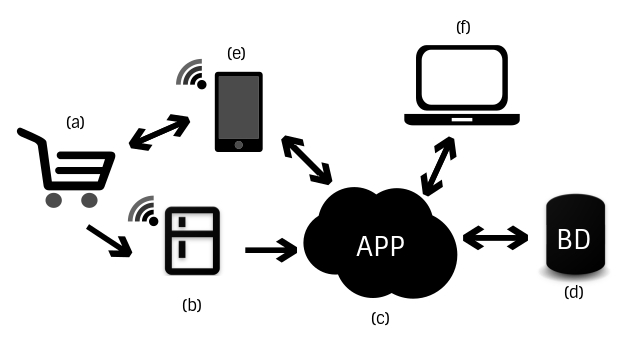
\includegraphics[width=16cm, height=8cm, scale=1]{./figures/architecture.png}
	\caption{Arquitetura Geral do Projeto}
	\label{project-general-architecture}
\end{figure}


A Figura \ref{project-general-architecture} representa o fluxo de dados entre os componentes envolvidos. Com a aquisição dos itens, estes são processados e armazenados nos seus respetivos locais de armazenamento, esta informação é enviada para a API. Estes dados são depois enviados e armazenados de forma persistente na \acrfull{bd}. Quando um dos \textit{endpoint}, \textit{mobile} ou \textit{web}, requisitam esses mesmos dados à API, estes são fornecidos pela \acrshort{bd}, tratados e devolvidos pela API. O fluxo de dados descendente dos \textit{endpoints} para a API acontece aquando o utilizador efetua manipulação de dados. A interação entre o \textit{smartphone} e os itens será posteriormente explicada.

%
% Secção 3.1 Abordagem
%
\section{Abordagem}\label{sec31}

No contexto do projeto assume-se a existência de duas formas de apresentação para os itens em stock: avulsos e embalados. Os primeiros são conservados em sistemas de arrumação identificados com \textit{tags} programáveis por \textit{smartphones}. Os detalhes dos itens são especificados pelo utilizador e carregados para a \textit{tag}. Enquanto que para os produtos embalados, admite-se que os produtores utilizam \textit{tags}, \acrfull{nfc} ou \acrfull{rfid}, para guardar os rótulos de forma digital e em formato standard.

Após a aquisição, os artigos são armazenados em locais que devem dispor de dispositivos de hardware equipados com leitores de \textit{tags}. É recolhida a informação presente na \textit{tag}, identificado o tipo de movimento (entrada ou saída) e enviado para a \gls{api-web}.

\begin{figure}[H]
	\centering
	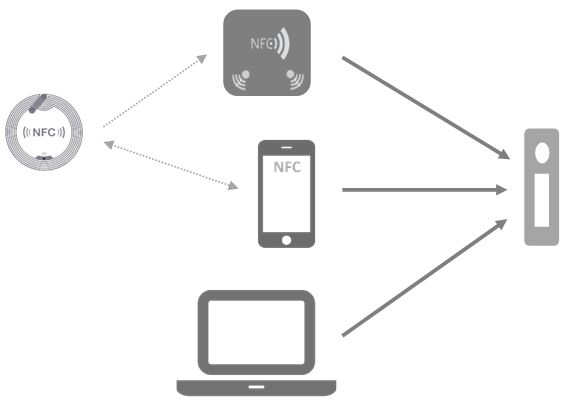
\includegraphics[height=9cm, scale=1]{./figures/project_structures.png}
	\caption{Estrutura do Lado do Cliente Projeto}
	\label{project-structure}
\end{figure}

\begin{figure}[H]
	\centering
	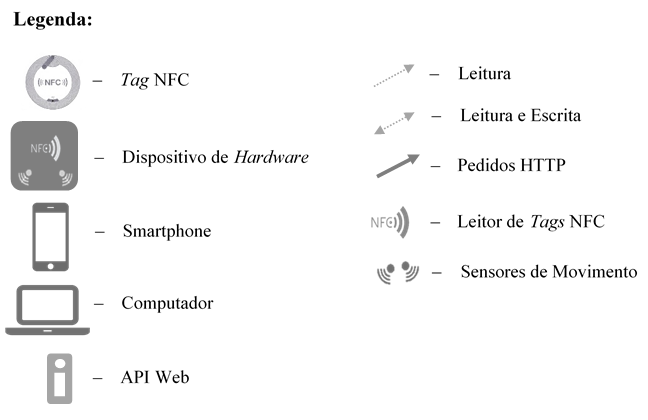
\includegraphics[height=9cm, scale=1]{./figures/project_structures_caption.png}
\end{figure}

Com a Figura \ref{project-structure} pretende-se não só apresentar os principais componentes do projeto, bem como demonstrar de forma breve a relação dos mesmos. É de destacar que uma \textit{tag} pode ser lida por um dispositivo de \textit{hardware} munido de um leitor de \textit{tags}. Assim como um \textit{smartphone}, equipado com tecnologia \acrshort{nfc}, pode escrever na \textit{tag} \acrshort{nfc}, tal é necessário para identificar produtos avulsos presentes num sistema de arrumação. Tanto o dispositivo de \textit{hardware} como as aplicações, móvel e \textit{web}, comunicam com a \gls{api-web}.\\

%
% Secção 3.2 Análise
%
\section{Análise}\label{sec32}

O projeto é composto por 2 blocos principais, que se relacionam. A Figura \ref{project-layers-structure} representa esses blocos. 

\begin{figure}[H]
	\centering
	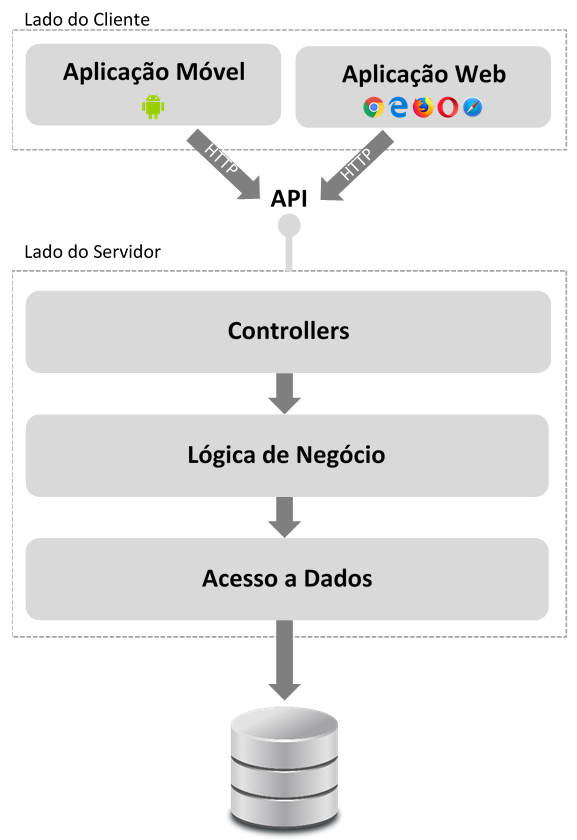
\includegraphics[height=9cm, scale=1]{./figures/project_architecture.png}
	\caption{Estrura por Camadas do Projeto}
	\label{project-layers-structure}
\end{figure}

O lado do servidor incluí quatro camadas e expõe uma \gls{api-web}. A camada da \acrfull{bd} é realizada com o \acrfull{sgbd} \textit{PostgreSQL}. A \acrfull{dal} é responsável pelas leituras e escritas à \acrshort{bd}. Esta camada é produzida com a linguagem de programação \textit{Java}, com a \acrfull{jpa}. A \acrfull{bll} é responsável pela gestão dos dados obtidos da \acrshort{bd} ou dos \textit{controllers}. A implementação desta camada recorreu à mesma ferramenta que foi usada na \acrshort{dal}. Os \textit{controllers} foram desenvolvidos em \textit{Java} com a \textit{framework} da \textit{Spring}, chamada de \textit{Spring Boot}. A \gls{api-web} disponibiliza recursos em diferentes \textit{hypermedia}.

Do lado do cliente existem dois modos de interação, por uma aplicação móvel e outra por uma aplicação web. A aplicação móvel disponível para a plataforma \textit{Android}, desenvolvida em linguagem \textit{Kotlin}. A aplicação web é disponibilizada para a maioria dos browsers, implementada utilizando a linguagem \textit{JavaScript}, com o auxilio da \textit{framework Express}.

%
% Secção 3.3 Dificuldades Encontradas
%
\section{Dificuldades Encontradas} \label{sec33}

Durante a investigação para a resolução deste projeto encontraram-se as seguintes dificuldades.

\subsection{Rótulos em Formato Não Digital}

Nos dias de hoje, os produtos não possuem rótulos digitais. Isto é um problema para a concretização do projeto, na medida em que se torna menos eficiente a recolha dos dados presentes nos produtos. Contudo, assumindo que este problema é resolvido fora do âmbito do projeto, apenas é preciso definir um formato standard de como os dados devem ser armazenados nas \textit{tags}, que podem ser \acrshort{nfc} ou \acrshort{rfid}. Num cenário ideal, este formato deve ser respeitado por todos os embaladores. Assim, os produtos têm um rótulo, código de barras e uma \textit{tag} \acrshort{nfc} ou \acrshort{rfid}, com a informação necessária. Está fora do âmbito do trabalho implementar o suporte hardware para a leitura das \textit{tags} e qual o sentido do movimento (entrada ou saída). Assume-se que essas informações são disponibilizadas num formato conhecido. 


\subsection{Ausência de Identificador Único nos Itens}

Os itens não dispõem de um identificador unívoco. Alguns deles contêm um lote e um número de série. A ausência deste identificador impede a distinção entre itens iguais, o que impossibilita saber se entrou um novo item no local de armazenamento ou se saiu um dos itens presentes. Tal facto torna a gestão dos stocks dependente do dispositivo de hardware para distinguir o tipo de movimento.
